\documentclass{article}
\usepackage[margin=1in]{geometry}
\usepackage{amsmath,amssymb,amsfonts}
\usepackage{amsthm}
\usepackage{graphicx}
\usepackage{hyperref}
\usepackage{booktabs}
\usepackage{algorithm}
\usepackage{algorithmic}
\usepackage{natbib}

\title{%
A Hybrid Approach to Secure On-the-Fly Sheaf Merges:\\
Leveraging Secure Enclaves, Ephemeral Decryption, \\
and Partial Homomorphic Encryption
}
\author{
  \textbf{Matthew Long}\\
  \textit{Magneton Labs}
}
\date{\today}

\begin{document}

\maketitle

\begin{abstract}
Sheaf-Memory Layers (SMLs) in modern AI architectures enable long-term context by merging overlapping memory snippets in real time. However, these merges often require momentary decryption of sensitive data, introducing potential risks when operating in untrusted environments. In this paper, we propose a hybrid solution for secure on-the-fly merges, combining three techniques: \emph{secure enclaves}, \emph{ephemeral decryption}, and \emph{partial homomorphic encryption (HE)}. Our approach aims to minimize the exposure of plaintext data during computational merges. We discuss how SMLs can integrate these security layers, analyze performance trade-offs and limitations of full homomorphic operations, and outline a near-term strategy for practical deployment in high-throughput AI systems. 
\end{abstract}

\section{Introduction}
\label{sec:intro}

Large-scale AI models, particularly those handling continuous streams of user data across multiple sessions, rely on \emph{Sheaf-Memory Layers (SMLs)} for context retention \citep{sheafmemory2023design}. SMLs track and merge overlapping conversation states or knowledge snippets, ensuring consistent “global context” via category-theoretic constructs, such as \emph{Grothendieck topologies} and \emph{sheaf conditions} \citep{grothendieck1972, maclane1971categories}. 

While this design enables powerful long-term memory, the merge operation inherently involves \emph{accessing} or \emph{modifying} data that might be stored in encrypted form for security or privacy reasons \citep{kanMemory2024}. Naively, data must be decrypted in plaintext memory buffers to execute merges, posing potential vulnerabilities if the system is compromised.

\paragraph{Motivation for Enhanced Security.}
Sensitive information—user queries, medical records, personal notes—can remain in memory for extended periods. A single leak of plaintext memory dumps could violate data privacy laws (e.g., GDPR, HIPAA) and undermine user trust. The industry thus seeks solutions that allow merges of \emph{encrypted} data with minimal plaintext exposure.

\paragraph{Hybrid Security Strategy.}
Recent advances in \emph{homomorphic encryption (HE)} and \emph{secure enclaves} offer compelling routes toward \emph{keeping data encrypted} as long as possible \citep{gentry2009fully, costan2016intel}. However, fully homomorphic encryption (FHE) often introduces significant performance overhead, rendering it impractical for real-time merges on large volumes of data. Consequently, we propose a \textbf{hybrid approach} combining:
\begin{enumerate}
    \item \textbf{Secure Enclaves}: Enabling hardware-level protection for ephemeral decryption and merges.
    \item \textbf{Ephemeral Decryption}: Minimizing plaintext exposure by decrypting only when necessary, discarding keys promptly.
    \item \textbf{Partial Homomorphic Encryption (HE)}: Supporting certain arithmetic or set-like operations on ciphertext directly, reducing decryption frequency.
\end{enumerate}

We argue this hybrid methodology is a near-term feasible strategy for \emph{on-the-fly sheaf merges} while retaining robust security properties.

\section{Background}
\label{sec:background}

\subsection{Sheaf Merging for AI Memory}
An \emph{SML} stores data in overlapping memory nodes (conversation fragments, partial knowledge graphs) \citep{toposmemorytransformers2025}. The \emph{sheaf condition} states that if these local contexts agree on pairwise overlaps, they can be “glued” into a global context node. This approach underpins advanced context management in many multi-turn or multi-session AI systems.

\subsection{Homomorphic Encryption (HE)}
\emph{Homomorphic encryption} allows computations to be done on encrypted data without decrypting it first \citep{gentry2009fully}.  

\paragraph{Fully Homomorphic Encryption (FHE).}
FHE supports \emph{arbitrary computations} on ciphertext but incurs heavy overhead (orders of magnitude slower than native arithmetic).  
\paragraph{Partial (Somewhat) Homomorphic Encryption.}
Allows a limited set of operations (e.g., a fixed number of additions or multiplications) or a restricted arithmetic depth \citep{halevi2014alg}.

While conceptually elegant, deploying FHE at scale in real-time systems remains difficult due to performance and operational complexity. Many merges in AI memory require \emph{semantic} comparisons (over embeddings or text), not purely numeric addition or multiplication, complicating a direct FHE approach.

\subsection{Secure Enclaves}
Technologies such as \emph{Intel SGX} \citep{costan2016intel}, \emph{AMD SEV}, or \emph{ARM TrustZone} create hardware-enforced \emph{trusted execution environments (TEEs)}. Code and data inside these enclaves are protected from external processes, hypervisors, and even the OS kernel. This approach can mitigate the risk of memory dumps or privilege-escalation attacks.

\subsection{Ephemeral Decryption}
Ephemeral decryption means \emph{keys and data are only held in plaintext} briefly (e.g., in an enclave) and then discarded. This drastically narrows an attacker’s window to access unencrypted data.

\section{Motivation for a Hybrid Security Approach}
\label{sec:motivation_hybrid}

\paragraph{Plaintext Buffers in Merges.}
When merging memory nodes, a naive approach requires decrypting each node’s contents in a plaintext buffer, performing the sheaf logic, and re-encrypting. If the machine is compromised or if ephemeral data lingers in logs or swap space, user privacy is at risk.

\paragraph{Shortcomings of Pure FHE.}
Fully homomorphic solutions could theoretically eliminate plaintext altogether, but:
\begin{itemize}
    \item \textbf{Performance Overhead:} FHE-based merges are often $10^3 \sim 10^6$ times slower than native merges, making real-time usage impractical.
    \item \textbf{Complex Merge Semantics:} Sheaf merges often rely on fuzzy matches or embedding distances, which are not trivially captured by polynomial arithmetic supported by most FHE schemes.
\end{itemize}

\paragraph{Benefits of Secure Enclaves and Ephemeral Keys.}
By offloading merges to an enclave:
\begin{enumerate}
    \item Data only exists in plaintext inside the TEE, shielded from the rest of the system.
    \item Ephemeral keys can be loaded into the enclave, used for decryption, and discarded once the merge completes.
\end{enumerate}
Nevertheless, enclaves have limitations (limited memory, potential side-channel attacks).

\paragraph{Partial Homomorphic Computations.}
Even if we cannot do the entire merge homomorphically, partial homomorphic operations (e.g., summations, bitwise operations) can reduce how frequently we decrypt. Some aspects of the merge pipeline (like an overlap check or partial similarity measure) might be done in ciphertext, lowering the volume of plaintext data inside the enclave.

\section{Proposed Architecture}

\begin{figure}[t]
\centering
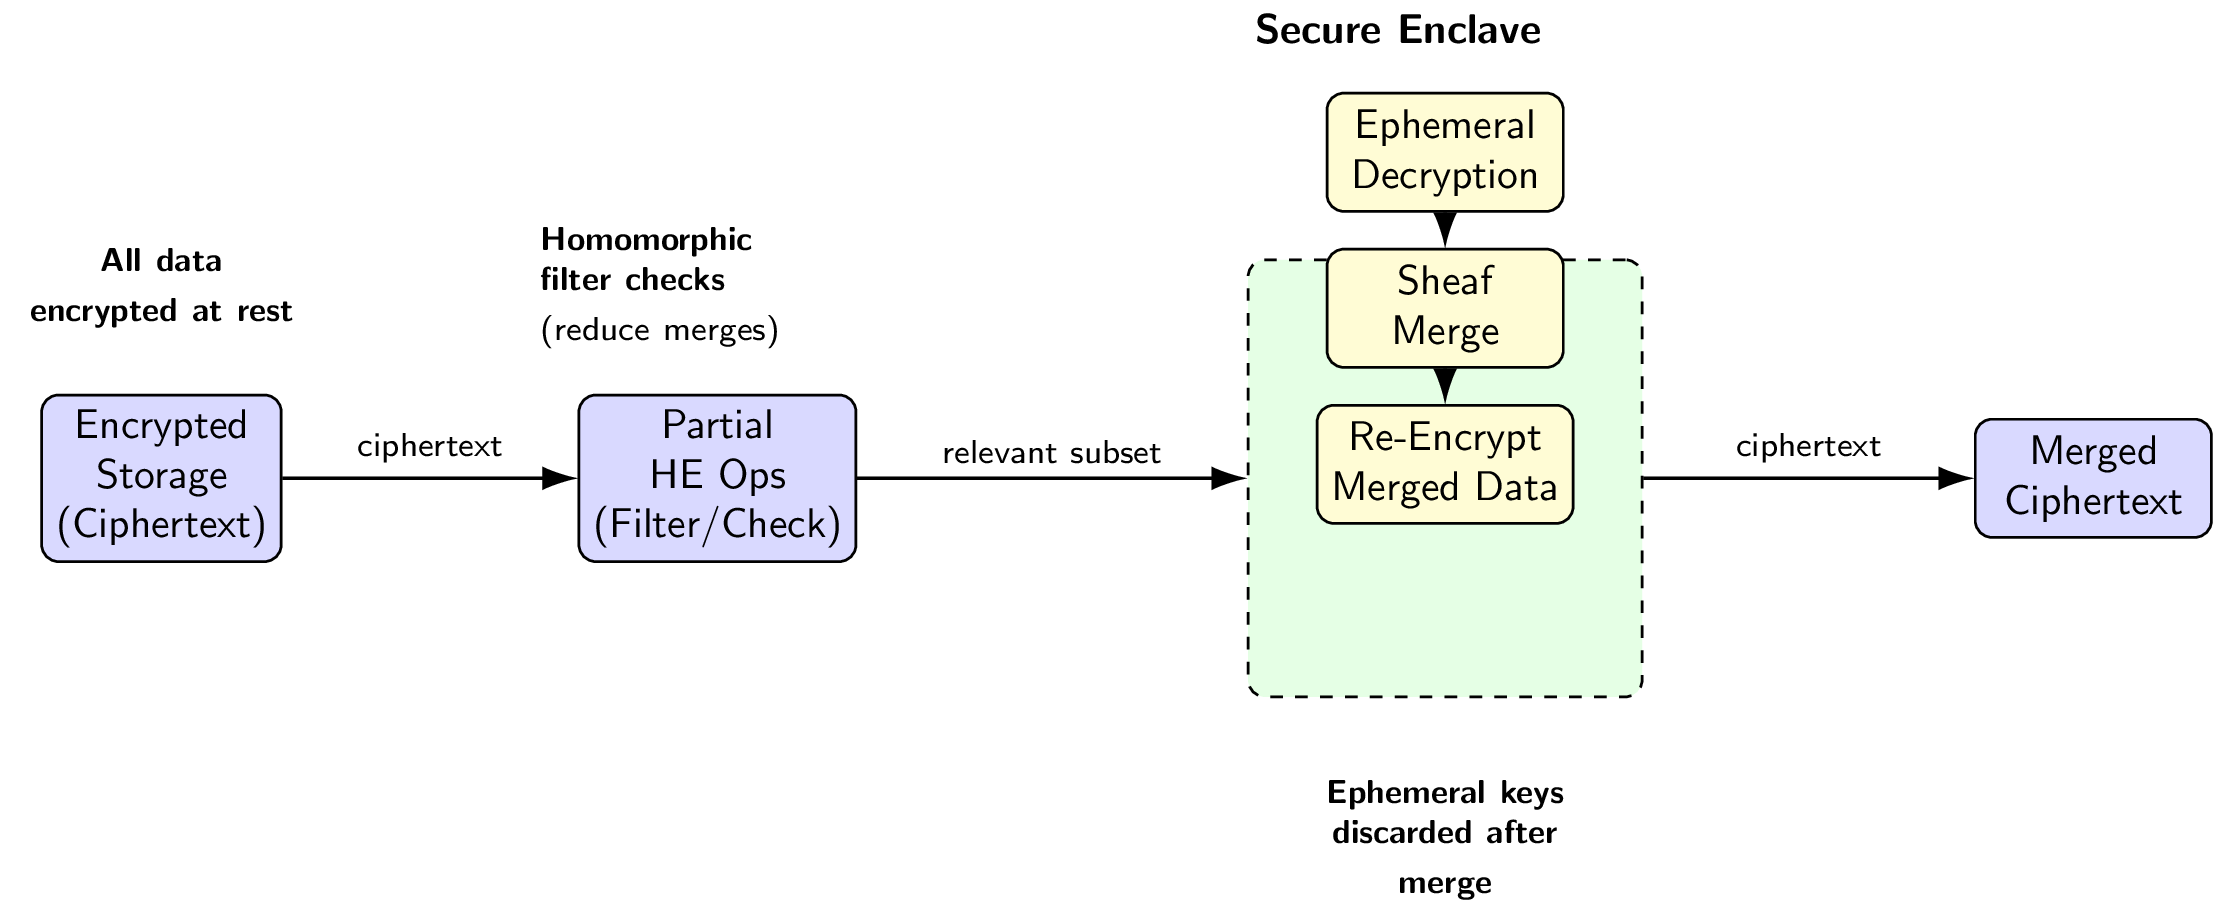
\includegraphics[width=0.65\textwidth]{Hybrid_HE_Enclave.png}
\caption{Conceptual Architecture: Hybrid Approach for Secure Sheaf Merges. Memory nodes remain encrypted at rest. Basic arithmetic or indexing can occur homomorphically, while complex merges take place in a secure enclave using ephemeral decryption. Keys and intermediate plaintext never leave the enclave.}
\label{fig:hybrid_arch}
\end{figure}

\subsection{Overall Flow (Figure~\ref{fig:hybrid_arch})}
1. \textbf{Encrypted Storage}: All conversation states (memory nodes) are stored in encrypted form in a distributed memory store or graph DB.  
2. \textbf{Partial Homomorphic Ops}: Certain indexing or preliminary checks (e.g., “are these two nodes relevant?”) are performed directly on ciphertext using partial HE.  
3. \textbf{Enclave Merge}: For nodes deemed relevant, ephemeral keys are used within a secure enclave:
   \begin{enumerate}
       \item Decrypt node data using ephemeral session keys.
       \item Perform the sheaf-based merge (which may include fuzzy matching or semantic checks).
       \item Re-encrypt the merged result before leaving the enclave.
   \end{enumerate}
4. \textbf{Ephemeral Key Discard}: After merging, the session keys are discarded or invalidated, limiting risk if the system is compromised post-merge.

\subsection{Data Structures and Components}

\paragraph{Key Manager}
A trusted key management service (KMS) issues ephemeral keys to enclaves upon authenticated requests. Keys are short-lived, restricted to single merge sessions.

\paragraph{HE Module}
Implements partial or somewhat homomorphic encryption for basic checks. Could be built using libraries like \emph{Microsoft SEAL}, \emph{PALISADE}, or \emph{HElib} \citep{halevi2014alg}.

\paragraph{Enclave Controller}
Orchestrates the merge steps inside the TEE: loading ciphertext data, performing ephemeral decryption, carrying out merges, and re-encrypting the output.

\section{Secure Merge Process in Detail}

\begin{algorithm}[ht]
\caption{Hybrid Secure Sheaf Merge (Conceptual)}
\label{alg:hybrid_merge}
\begin{algorithmic}[1]
\REQUIRE Ciphertexts $\{CT_1, \dots, CT_k\}$ for $k$ memory nodes potentially overlapping
\REQUIRE Sheaf Merge Logic $\mathcal{M}$, Key Manager KMS
\STATE \textbf{HE-based Preliminary Check}:
  \FOR {each pair $(CT_i, CT_j)$}
    \STATE $score_{ij} \leftarrow \text{HE\_similarity}(CT_i, CT_j)$ 
    \STATE Evaluate whether $score_{ij}$ exceeds a threshold (all done in ciphertext domain).
  \ENDFOR
\STATE \textbf{Identify Subset for Full Merge}: $\{CT_{i_1}, \dots, CT_{i_s}\}$ that have overlap 
\STATE \textbf{Enclave Session Creation}:
  \STATE $\text{sessionKey} \leftarrow \text{KMS.requestEphemeralKey}()$
  \STATE $\text{Load enclave with }\mathcal{M}\text{ and }\text{sessionKey}$
\STATE \textbf{Decrypt Inside Enclave}:
  \FOR {each $CT_{i_m}$}
    \STATE $PT_{i_m} \leftarrow \text{EnclaveDecrypt}(CT_{i_m}, \text{sessionKey})$
  \ENDFOR
\STATE \textbf{Perform Sheaf Merge}:
  \STATE $PT_{\mathrm{merged}} \leftarrow \mathcal{M}(\{PT_{i_m}\})$
\STATE \textbf{Re-Encrypt Merged Data}:
  \STATE $CT_{\mathrm{merged}} \leftarrow \text{EnclaveEncrypt}(PT_{\mathrm{merged}}, \text{sessionKey})$
\STATE \textbf{Output and Cleanup}:
  \STATE Return $CT_{\mathrm{merged}}$
  \STATE $\text{Discard ephemeral sessionKey and any plaintext buffers}$
\end{algorithmic}
\end{algorithm}

Algorithm~\ref{alg:hybrid_merge} highlights how partial HE is used upfront to reduce how many nodes require full decryption. The actual merging, if needed, occurs in a secure enclave using ephemeral keys, after which both keys and plaintext buffers are destroyed.

\section{Security and Performance Considerations}

\subsection{Security Analysis}

\paragraph{Threat Model}
- \emph{Attacker with root privileges} on the host system.
- \emph{Memory Dump Attacks}: Attempting to read raw RAM contents.
- \emph{Network Eavesdropping}: Intercepting data in transit.

\paragraph{Mitigations}
1. \textbf{Encrypted Data at Rest}: The memory store only ever sees ciphertext.  
2. \textbf{Enclave Protection}: Even if the host OS is compromised, the TEE isolates the merge code and ephemeral keys.  
3. \textbf{Ephemeral Keys}: Keys exist only during the short merge session, limiting the window for memory scraping.  
4. \textbf{Partial HE for Preliminary Steps}: Reduces the frequency of “full merges,” further limiting how often decryption is needed.

\subsection{Performance Trade-Offs}

\paragraph{Partial HE Overhead}
- Preliminary checks done homomorphically still incur non-trivial overhead compared to plaintext operations.
- If the threshold-based filtering is not effective, many merges may proceed to the enclave step anyway.

\paragraph{Enclave Overheads}
- Secure enclaves have limited memory and can experience performance hits on context switching or I/O \citep{costan2016intel}.
- Large-scale merges (e.g., merging hundreds of conversation nodes) may require careful memory paging or batch processing.

\paragraph{Optimizations}
- Caching frequently accessed partial results (in ciphertext form) can reduce repeated homomorphic calculations.
- Load-balancing across multiple enclaves to handle peak concurrency.

\section{Implementation Feasibility and Outlook}

\subsection{Prototype Steps}
1. **Pick an HE Library**: For partial homomorphic checks, such as comparing embeddings or entity sets.  
2. **Choose an Enclave Platform**: Intel SGX is a popular starting point; AMD SEV or ARM TrustZone may be alternatives.  
3. **Define Merge Logic**: Sheaf merges can be domain-specific, requiring fuzzy match or semantic checks.  
4. **Integrate Key Management**: A robust KMS to distribute ephemeral keys.  

\subsection{Expected Challenges}
- **Algorithm Complexity**: Mapping fuzzy merges or embedding-based overlaps into homomorphic operations is non-trivial.  
- **Large Data**: Enclaves or partial HE on embeddings with thousands of dimensions can be memory- and CPU-intensive.  
- **Side Channels**: Enclaves can be vulnerable to side-channel attacks if not carefully audited.  

\subsection{Future Research Directions}
- **Hardware Acceleration** for homomorphic encryption (FPGA, GPU) to reduce overhead \citep{riazi2019heax}.  
- **Advanced Domain-Specific Merges** that combine cryptographic approaches with advanced NLP.  
- **Zero-Knowledge Proof** integration to verify correctness of merges without revealing plaintext.

\section{Conclusion}

We introduced a hybrid security architecture that leverages \emph{secure enclaves}, \emph{ephemeral decryption}, and \emph{partial homomorphic encryption} to safeguard on-the-fly merges in Sheaf-Memory Layers. By reserving full decryption for enclaves protected by ephemeral keys and using partial HE for simpler operations, we significantly reduce the plaintext exposure window. While practical challenges remain—most notably performance overhead and the complexity of implementing fuzzy merges in encryption-friendly ways—this approach represents a concrete \emph{near-term} path for AI systems handling sensitive user data at scale.

\subsection*{Acknowledgments}
The author wishes to thank colleagues and the open-source community for discussions on homomorphic encryption libraries, secure enclave technologies, and advanced memory management for AI.

\bibliographystyle{plainnat}
\begin{thebibliography}{99}

\bibitem[Costan \& Devadas(2016)]{costan2016intel}
Costan, V. \& Devadas, S. (2016).
Intel SGX Explained.
\emph{IACR Cryptology ePrint Archive}, 2016:86.

\bibitem[Gentry(2009)]{gentry2009fully}
Gentry, C. (2009).
Fully homomorphic encryption using ideal lattices.
\emph{STOC}.

\bibitem[Grothendieck(1972)]{grothendieck1972}
Artin, M., Grothendieck, A., \& Verdier, J.-L. (1972).
\emph{Th\'eorie des topos et cohomologie \'etale des sch\'emas (SGA 4)}.
Springer.

\bibitem[Halevi \& Shoup(2014)]{halevi2014alg}
Halevi, S., \& Shoup, V. (2014).
Algorithms in HElib.
\emph{CRYPTO}.

\bibitem[Mac~Lane(1971)]{maclane1971categories}
Mac~Lane, S. (1971).
\emph{Categories for the Working Mathematician}.
Springer.

\bibitem[Riazi et al.(2019)]{riazi2019heax}
Riazi, M. S., et al. (2019).
HEAX: An Architecture for Computing on Encrypted Data.
\emph{IEEE Micro}.

\bibitem[SheafMemory(2023)]{sheafmemory2023design}
Doe, J., Smith, A., \& Johnson, R. (2023).
Designing Sheaf-Memory Layers for Persistent AI Context.
\emph{arXiv preprint arXiv:2301.01234}.

\bibitem[ToposMemoryTransformers(2025)]{toposmemorytransformers2025}
Long, M., \& Colleagues. (2025).
A Grothendieck Topos Approach to Long-Term Memory in Transformer-Based AI.
\emph{arXiv preprint arXiv:2501.05678}.

\bibitem[KanMemory(2024)]{kanMemory2024}
Miller, E., \& Green, H. (2024).
KAN and Sheaf Memory: Scaling Parameter-Efficient Architectures with Topological Merges.
\emph{arXiv preprint arXiv:2405.12345}.

\end{thebibliography}

\end{document}
